\documentclass[]{elsarticle} %review=doublespace preprint=single 5p=2 column
%%% Begin My package additions %%%%%%%%%%%%%%%%%%%
\usepackage[hyphens]{url}

  \journal{Materials Today: Proceedings} % Sets Journal name


\usepackage{lineno} % add
  \linenumbers % turns line numbering on
\providecommand{\tightlist}{%
  \setlength{\itemsep}{0pt}\setlength{\parskip}{0pt}}

\usepackage{graphicx}
\usepackage{booktabs} % book-quality tables
%%%%%%%%%%%%%%%% end my additions to header

\usepackage[T1]{fontenc}
\usepackage{lmodern}
\usepackage{amssymb,amsmath}
\usepackage{ifxetex,ifluatex}
\usepackage{fixltx2e} % provides \textsubscript
% use upquote if available, for straight quotes in verbatim environments
\IfFileExists{upquote.sty}{\usepackage{upquote}}{}
\ifnum 0\ifxetex 1\fi\ifluatex 1\fi=0 % if pdftex
  \usepackage[utf8]{inputenc}
\else % if luatex or xelatex
  \usepackage{fontspec}
  \ifxetex
    \usepackage{xltxtra,xunicode}
  \fi
  \defaultfontfeatures{Mapping=tex-text,Scale=MatchLowercase}
  \newcommand{\euro}{€}
\fi
% use microtype if available
\IfFileExists{microtype.sty}{\usepackage{microtype}}{}
\bibliographystyle{elsarticle-harv}
\ifxetex
  \usepackage[setpagesize=false, % page size defined by xetex
              unicode=false, % unicode breaks when used with xetex
              xetex]{hyperref}
\else
  \usepackage[unicode=true]{hyperref}
\fi
\hypersetup{breaklinks=true,
            bookmarks=true,
            pdfauthor={},
            pdftitle={Sustainable 3D printing using recycled PLA: A comparative study based on the mechanical resistance},
            colorlinks=false,
            urlcolor=blue,
            linkcolor=magenta,
            pdfborder={0 0 0}}
\urlstyle{same}  % don't use monospace font for urls

\setcounter{secnumdepth}{5}
% Pandoc toggle for numbering sections (defaults to be off)

% Pandoc citation processing
\newlength{\csllabelwidth}
\setlength{\csllabelwidth}{3em}
\newlength{\cslhangindent}
\setlength{\cslhangindent}{1.5em}
% for Pandoc 2.8 to 2.10.1
\newenvironment{cslreferences}%
  {}%
  {\par}
% For Pandoc 2.11+
\newenvironment{CSLReferences}[3] % #1 hanging-ident, #2 entry spacing
 {% don't indent paragraphs
  \setlength{\parindent}{0pt}
  % turn on hanging indent if param 1 is 1
  \ifodd #1 \everypar{\setlength{\hangindent}{\cslhangindent}}\ignorespaces\fi
  % set entry spacing
  \ifnum #2 > 0
  \setlength{\parskip}{#2\baselineskip}
  \fi
 }%
 {}
\usepackage{calc} % for calculating minipage widths
\newcommand{\CSLBlock}[1]{#1\hfill\break}
\newcommand{\CSLLeftMargin}[1]{\parbox[t]{\csllabelwidth}{#1}}
\newcommand{\CSLRightInline}[1]{\parbox[t]{\linewidth - \csllabelwidth}{#1}}
\newcommand{\CSLIndent}[1]{\hspace{\cslhangindent}#1}

% Pandoc header



\begin{document}
\begin{frontmatter}

  \title{Sustainable 3D printing using recycled PLA: A comparative study
based on the mechanical resistance}
    \author[University of Jaén]{V.M. López\corref{2}}
   \ead{alice@example.com} 
    \author[University of Vigo]{Diego Carou}
   \ead{diecapor@uvigo.es} 
    \author[Université de Lorraine, ERPI, F-54000 Nancy, France]{Fabio
A. Cruz Sanchez\corref{1}}
   \ead{cruzsanc1@univ-lorraine.fr} 
      \address[Department of Mechanical and Mining Engineering]{Campus
Las Lagunillas, 23071 Jaén, Spain}
    \address[Department of Design in Engineering]{Campus As Lagoas,
32004 Ourense, Spain}
      \cortext[1]{Corresponding Author}
    \cortext[2]{Equal contribution}
  
  \begin{abstract}
  Nowadays, sustainability is one of the major objectives for
  manufacturing. The use of recycled materials can be a suitable
  strategy when economic, environmental and technical feasibility are
  verified. 3D printing is still a novel manufacturing process and the
  research on the topic is still limited, particularly when referring to
  sustainability issues. This paper attempts to evaluate the suitability
  of the substitution of virgin PLA by recycled PLA. To do that, it
  includes an experimental plan divided into three phases including ..
  to evaluate the technical feasibility based on mechanical resistance.
  The results showed that recycled PLA may be used due to the, though
  slightly lower, similar mechanical resistance than that of the virgin
  material. This reduction is limited to 13 \% in the worst
  configuration (vertical). Besides, it was identified how the infill
  density and the orientation used for printing played a major role on
  the mechanical resistance, when others such as the infill pattern,
  printing speed and layer height had non-significant influence.
  \end{abstract}
  
 \end{frontmatter}

\hypertarget{introduction}{%
\section{Introduction}\label{introduction}}

Additive manufacturing (also called 3D printing) is becoming a key
technology for a cross domains applications. The layer-by-layer
principle enables a higher flexibility degree in the product design
phase {[}ref{]}. This technology is pushing forward advantages such as
customization of objects of complex geometries with a great deal of
detail, combination of different materials, no need for assembly and
high utilization rate of raw materials ( Jin et al.~(2017); Xiao et al.,
2014). Thus, the technology is receiving great attention by companies
and genereal public.

3D printing has developed significantly over time. A great development
is expected in sectors such as product consumption, medical products and
aerospace components (Peng et al., 2018).The rapid prototyping market
reached \$7.3 billion US dollars in 2018 according to Wohlers
(Rodriguez-Hernández et al., 2020), which also forecasts the market to
reach 23.9 and 35.6 billion dollars by 2022 and 2024, respectively
(Forbes, 2019). The industry has grown from \$295 million to 5.1 billion
over the past 25 years. Nowadays, there is a need to find paths to
reduce the ecological impact that manufacturing processes (including 3D
printing technology) have is an important topic addressed by a large
number of researchers {[}ref{]}. Research efforts to identify
opportunities of 3D printing on the circular economy paradigm start to
be explored {[}1{]}. Plastic is one of the most used materials in the 3D
printing industry, and given their non-biodegradable nature, it is one
the most abundant type of waste produced and their impact is well
document in the different ecosystems {[}ref{]}. Thus, reducing the
consumption of plastics and/or the use of the plastics already presented
in the ecosystem is of great importance for the environment. To this
purpose, distributed recycling via additive manufacturing approach
methodology make an emphasis in the technical steps to possible reuse
plastic waste through the recyling chains for material extrusion based
techniques of 3D printing {[}3{]}. In the DRAM methodology, consumers
have an economic incentive to recycle because they can use their waste
as feedstock for a wide range of consumer products that can be produced
for a fraction of conventional costs of equivalent products. Moreover,
3D printing is especially suited because it allows producing parts with
almost no waste (Sehdev et al., 2017) and could reduce more than 40 \%
of the waste related to the used material, reusing 95 \% of the unused
material (Petrovic et al.~2011). Nevertheless, one of the the systemic
problem of plastic waste relies on dependency of the indiscriminate
disposal of plastics which carries multiple risks because many plastic
products contain additives that modify their physico-mechanical
properties difficulting their recycling/reuse {[}4{]}. The use of
biopolymers of natural and renewable origin promising strategies to
alleviate these problems (Zhao et al., 2018a) (Bhatia and Ramadurai,
2017) (Liu et al., 2018). However, the number of publications is limited
when it comes to sustainable manufacturing using 3D printing (Peng et
al., 2018). Although the technology offers high efficiency in the use of
material, the great democratization of this technology could cause a
feedback impact due to the increasing generation and disposal of huge
amounts of waste or polluting emissions to fabricated virgin feedtock.
Currently, most of the cost of 3D printing is associated with the cost
of the filament {[}ref{]}. By recycling raw materials such as polylactic
acid (PLA), the emissions of carbon dioxide can be reduced in the
transport to landfills or shipping to customers offering environmental
benefits {[}ref{]}. The technical feasiblity for recycling in laboratory
conditions been proved for PLA {[}5{]}, ABS {[}6{]}, PET {[}7{]} that
recycled plastics have a similar performance to their virgin
counterparts and they have even been applied in the manufacture of high
value products in some sectors such as the automobile (Zhao et al.,
2018a). However, studies on the technical acceptability of recycled
materials as substitutes for conventional virgin materials are still
limited for particular applications \ldots{} The present study evaluates
the mechanical properties of both conventional and recycled PLA
specimens. The objective of the study is the assessment of the
suitability of the recycled PLA as replacement to advance to more
sustainable 3D printing processes. To do that, the study analyzed the
influence of several printing parameters on the mechanical properties of
the parts based on a comprehensive experimental program. Then, a printed
parts was designed comparing with a virgin to evaluate the acceptability
in \ldots{}

\hypertarget{literature-review}{%
\section{Literature review}\label{literature-review}}

One of the most common processes in 3D printing is the fused deposition
modeling (FDM) process. The process is based on material extrusion, so
the material is heated above the melting point of the material and then
deposited onto a platform (Wolszczak et al., 2018). In FDM, a variety of
thermoplastic materials are commonly used, such as acrylonitrile
butadiene styrene (ABS), polyvinylchloride (PVS), polycarbonate (PC),
nylon, polifenilsulfona, high density polyethylene (HDPE), low density
polyethylene (LDPE), polyethylene terephthalate (PET), high impact
polystyrene (HIPS) and polylactic acid (PLA) (Chua et al., 2017) (Zhao
et al., 2018b) (Kumar and Singh, 2018).

The development of new materials such as polymers, elastomers and
composites in engineering plays a fundamental role in the advance
sustainable manufacturing (Ashby and Johnson 2010). The use of
biopolymers of natural and renewable origin, replacing synthetic
polymers, is the cellulose, hemicellulose, lignin, starch, alginate,
chitosan and derivatives derived from them represent the most abundant
bio-based and renewable raw materials for different 3D printing
technologies. In addition, these biopolymers of natural origin include
lignocellulosic materials, seaweed materials and exoskeleton crustacean
materials (Liu et al., 2018). Liu et al.~(2018) reviews a wide range of
biobased printing materials with the adequate printing/solidification
approach and printed structures and potential applications. Most of them
find potential applications in biomedicine such as Cellulose nanofibers
(CNF)/alginate and Methylcellulose alginate that have as potential
applications cartilage tissue engineering and regenerative therapy,
respectively. To print biological matter, new 3D printing methods, such
as cryolithography, are appearing. These methods find applications in
tissue engineering and food engineering (Zawada et al.~(2018)).

Polylactic acid is a type of natural biopolymer obtained from crops such
as starch or sugar cane. It is a biodegradable biopolymer constituted of
lactic acid molecules and it is one of the most used materials in 3D
printing. In addition, PLA is a sustainable alternative that shows a
range of crystallinity and mechanical properties between polystyrene and
polyethylene terephthalate (Kumar et al., 2018) (Zhao et al., 2018b).

Recycling (mixing of virgin material with used material) of raw material
is a method of special interest to contribute to manufacture in a
sustainable way (Zhao et al., 2018a). However, it is important to
evaluate the properties of the recycled materials before substituting
virgin for recycled materials.

In this sense, Kumar et al.~(2018) compared the elongation at break,
load at break, flow index, Young's module and breaking stress of
recycled ABS, high impact polystyrene (HIPS) and PLA. The PLA showed the
highest elongation at break along with the ABS. In addition, the PLA had
a higher breaking load and breaking stress, although a smaller Young's
modulus. Other authors such as Gu et al.~(2016) identified the
suitability of using recycled polypropylene instead of virgin
polypropylene based on mechanical properties. Specifically, they found
that the use of fillers (talc and glass fibre) improved the mechanical
properties. Babagowda et al.~(2018) studied the influence of the
percentage of recycled PLA used in the filament (i.e., 10 to 50 \%)
showing that the smaller the percentage the higher the ultimate tensile
strength. Pinho et al.~(2020) obtained higher values of tensile stress
for recycled PLA when comparing to the virgin one. Nur-A-Tomal et
al.~(2020) presented a paper to evaluate the reusing of waste children's
toys as raw material for 3D printing.

As Suárez and Domínguez (2020) pointed out, the use of recycled
materials is still uncertain because the potential changes in the
material properties then recycling. Zhao et al.~(2018a) studied the
cycles of printing that is able to withstand the PLA until it loses much
of its properties. Thus, they showed that PLA withstands two printing
cycles, since in a third cycle the mechanical properties and viscosity
decreased considerably. The increase in crystallinity and melting
enthalpy and the decrease of cold crystallization enthalpy are
attributed to the 3D printing process, not to the extrusion recycling
process. Table 1 shows the comparison of the properties between the
virgin material and the same material subjected to another printing
cycle, being possible to appreciate how properties such as the tensile
strength and modulus are close for the two materials. Similarly, other
authors such as Lanzotti et al.~(2019) have proved how recycling PLA
provides comparable mechanical properties as the virgin material only
after a second recycling process.

The recycling of PLA has certain limitations because of reducing
molecular weight with its reuse, resulting in degradation and decrease
of mechanical properties. For instance, the addition of polidopamine
(PDA) on the surface allows improving these properties. Viscosity is
also reduced with each printing cycle but, it could be corrected by
adding virgin plastic (Zhao et al., 2018a) (Zhao et al., 2018b). When
recycling, there is a decrease in the properties of the material as a
result of the presence of carbonyl groups and superficial pitting due to
thermomechanical degradation during the process of new melting process
occurring during 3D printing (Zhao et al., 2018a).

The mechanical properties of the parts are critical for engineering
parts, particularly, for 3D printed parts. Several studies evaluated the
mechanical properties of 3D printed parts for various materials; Popescu
et al.~(2018) reviewed some of them in their study. The printing
conditions used to manufacture the parts have an important role on the
obtained results. So, it is important to identify the most important
parameters among all of the available to carry out the process that may
affect the response variable and their expected influence based on the
scientific literature (Sheoran and Kumar, 2020). For instance, Popescu
et al.~(2018) determined that the key parameters that influence the
mechanical properties in 3D printing are porosity, layer height, filling
density, printing direction and part orientation. In addition, for low
values of layer height, as well as the thickness of the deposited or
printed filament, the tensile strength of the material is improved. In
addition, by orienting the printing direction towards the direction in
which the tensile load will be applied during tensile strength, the
property can be also maximized. The importance of the printing
orientation was also identified by Yao et al.~(2019). According to
Alafaghani and Qattawi (2018), a higher extrusion temperature and an
optimized layer thickness, a triangular filling pattern and a higher
filling level maximize the strength of the parts. Regarding the printing
speed, it is identified that higher printing speed with higher layer
thickness result in lower part strength.

Among others, Altan et al.~(2018) also identified the influence of the
layer height on the mechanical resistance.

Nevertheless \ldots{}

\hypertarget{experimental-procedure}{%
\section{Experimental procedure}\label{experimental-procedure}}

\hypertarget{materials-and-equipement}{%
\subsection{Materials and equipement}\label{materials-and-equipement}}

The printing materials used in the study were virgin and recycled PLA
characterized by data listed in Table S1. Both materials were commercial
ones, so the recycling was not done during the research. The recycled
PLA contained 10 \% of virgin PLA in the blend.

The 3D printer used to manufacture the specimens was a BQ's Witbox,
shown in Fig1a. The software used to generate the printing code was the
Ultimaker Cura 3.2.1. To perform the destructive test, the machine used
was the MTS Criterion 43 universal testing machine (MTS, 2020) (Fig 1b)
with a maximum load of 50 kN, being the maximum load supported by the
LPS 104 cell of 10 kN. The clamping system was the Instron 2716-015
system with a maximum supported load of 30 kN. The selected strain rate
was 0.5 mm/min.

In order to save material and time to carry out the experimental plan,
the geometry of the specimen was reduced in size from the one
recommended by the UNE 116005:2012 standard (UNE, 2012), which define
the length of the specimen at no less than 120 and 150 mm depending on
the orientation. However, in this study the specimens are manufactured
according to the dimensions proposed by Lin et al.~(2018) in which the
length of the specimen was 75 mm. The dimensions of the specimen are the
ones depicted in Fig. 2.

\hypertarget{methodology}{%
\subsection{Methodology}\label{methodology}}

The aim of the study is identifying the most critical factors affecting
the mechanical properties in 3D printing, evaluating their influence on
the mechanical properties in 3D printing, particularly for both virgin
and recycled PLA. Thus, based on the results, it is expected to gain a
better understanding on the suitability of using recycled materials in
3D printing and how to properly select the printing conditions to
guarantee sufficient mechanical resistance. In order to do that, an
experimental plan comprising three phases will be developed.

Based on the literature research, the critical parameters for the study
are the (1) layer height and (2) infill pattern. In addition, taking
into account the goal of sustainable manufacturing (i.e., trying to
optimize the consumption of material), but also productivity (i.e.,
trying to minimize printing times), infill density and printing speed
were considered (Singh et al., 2018; Tanveer et al., 2019). The response
variable chosen was the maximum load attained during the testing of the
specimen ((Kumar et al., 2018), (Chacon et al., 2017); (Letcher et al.,
2015)).

The experimental plan included three different phases (Figure 2) to
carry out a comprehensive study with a limited number of tests not
compromising the reliability of the results.

In Phase I, the objective was to identify which were the most important
factors that have influence on the response variable. The Phase II
allowed studying in more detail the influence of the most influential
factors according to phase I. Finally, the Phase III aimed at evaluating
the influence of the anisotropy of the specimens depending on the
printing orientation, which may notably affect the mechanical resistance
of the specimen. Table S2 summarizes the tests of three phases.

In Phase I, the factors analyzed were those identified in previous
sections as critical. Thus, layer height, infill pattern, infill density
and printing speed were selected using two levels for each of them, with
large ranges, especially for the infill density. Thus, the factors and
their levels used were: layer height (0.15 and 0.3 mm), infill pattern
(tri-hexagonal and grid) , infill density (60 and 100 \%) and printing
speed (40 and 80 mm/s). The printing temperature chosen was 210 °C,
which was the recommended one for these materials.

Fractional designs are useful for reducing the number of tests reducing
time and money (Montgomery, 2001), being use as screening designs. So,
in order to identify and discard factors depending on their influence
with a limited number of tests, phase I recurred to fractional designs.
The design included only specimen printed in the horizontal orientation
for each of the combinations, not evaluating the influence of the
orientation, in order to save time and material. The use of random order
allowed guaranteeing that the hypothesis that the errors are
independently distributed random variables was fulfilled (Montgomery,
2001).

Phase II depended on the results of the previous phase. In this phase,
the most influential parameter of the ones studied in Phase I (note: the
factor resulted to be the infill density) was evaluated in more detail.
The selection of levels for the other three factors aimed at minimizing
the printing time. Thus, the selection of the factors was layer height
of 0.3 mm, infill pattern tri-hexagonal and printing speed of 80 mm/s
with an estimated printing time of 20 min. Regarding the infill density,
five levels were chosen ranging from 40 to 100 \% to evaluate the
evolution of the maximum load versus the infill density for both virgin
and recycled PLA. The specific levels selected were 40, 55, 70, 85 and
100 \%.

Phase III aimed at analyzing the influence of the orientation. Because
of the anisotropy, the UNE 116005:2012 (UNE, 2012) standard requires
printing specimens in three different orientations: edgewise (E),
horizontal (H) and vertical (V), testing five samples in each
orientation. The selected printing conditions were infill density of 50
\%, printing speed of 80 mm/s, tri-hexagonal infill pattern and layer
height of 0.3 mm, with the objective of limiting the use of material and
the time required for printing. In total, the phase included the
printing of 15 specimens of each virgin and recycled PLA.

\hypertarget{results-and-discusions}{%
\section{RESULTS AND DISCUSIONS}\label{results-and-discusions}}

Table S3 lists all the maximum load results attained during testing.

\hypertarget{phase-i-screening-phase}{%
\subsection{Phase I: Screening phase}\label{phase-i-screening-phase}}

In general, shortly after attaining the maximum load, the fracture of
the specimen occurred. However, the nature of the fracture was not
homogenous as shown in Fig 4. Thus, in most cases, the specimens showed
a fragile behavior and the fracture, either horizontally or with a lower
inclination angle, is clean. However, for the recycled material, the
specimens showed a ductile behavior and, properly, the fracture did not
occur after the maximum load was attained, canceling the tests minutes
after the maximum load was attained. The breakage in these cases
occurred at a 45º angle and, in the cases of the RE-2 specimen, two
parallel fracture lines can be clearly seen. The printing conditions did
not allow seen a clear relation to the fracture of the specimens. This
behavior may relate to that explained by Yao et al.~(2020). The authors
identified two different types of fracture: in-layer and interlayer. In
general, the fracture occurs at the interface of two layers when
printing in vertical position, even when varying the printing
orientation up to 45º from the vertical position. In-layer fracture is
more likely when the specimen is printed using an edgewise position (or,
inclined up to 45º from that position). In this second case, the
printing direction is the same as the tensile stress direction, which
also happens when the horizontal orientation is used. In these cases,
the material layer is not intact after the fracture.

Thus, it is likely that both modes coexist in this study, which may
explain the heterogeneity of the different fractures.

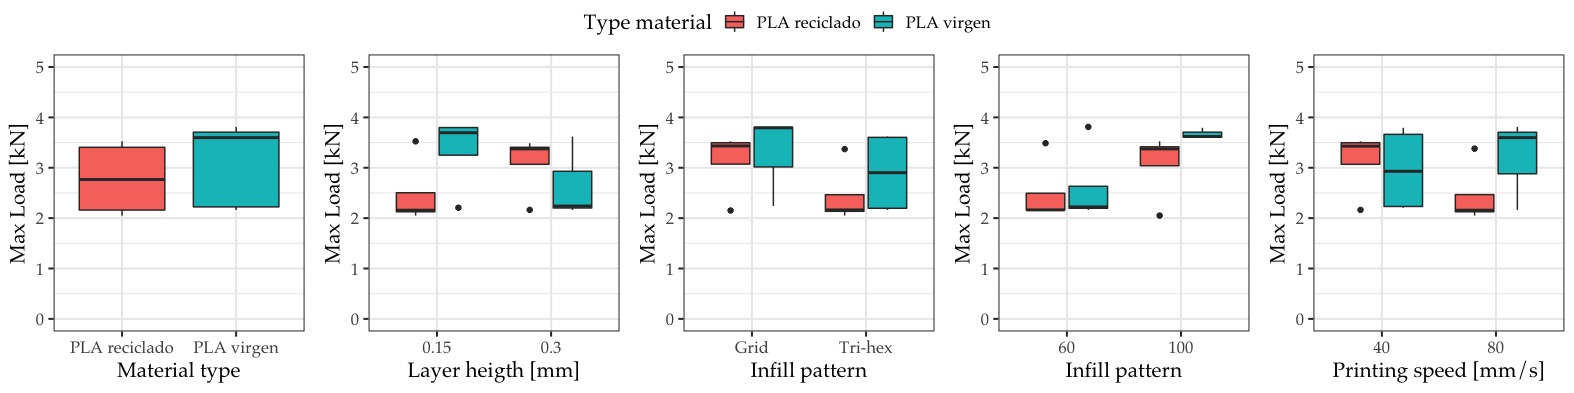
\includegraphics[width=21.86in]{Figures/Phase.1}

The analysis of variance (ANOVA) performed using R software allowed
identifying the influential factors on the response variables. As
criterion, critical factors for the response variable were those with
p-values lower than 0.05 (Pérez et al., 2018). Shapiro-Wilk normality
tests allowed verifying the normality of the residuals. Table 2 lists
the results of the ANOVAs carried out for both virgin and recycled PLA.

From Table 2, it can be clearly identified how only the infill density
was a statistically significant factor for the maximum load for both
materials (p-valor lower than 0.001). When evaluating the contribution
of each of the factors to the variability explained by the model, there
were calculated values of 99.30 \% and 99.85 \% for virgin and recycled
PLA, respectively. Thus, when manufacturing new parts or specimens,
infill density is a key factor for guarantying adequate mechanical
properties of the specimens. A new ANOVA allowed evaluating the
influence of the material on the maximum load, maintaining the sources
of variation previously analyzed. Table S4 shows the obtained results.
When including the material in the ANOVA, infill density is still the
most influential factor. However, in this case, the type of material is
also a significant factor for the response variable, being
non-significant the rest of the factors. Though significant, when
assessing the contribution of the material to the variability of the
model, it only accounted for 1.25\% of this variability, as shown in
Figure S1.

\hypertarget{phase-ii-evaluation-of-the-infill-density-influence}{%
\subsection{Phase II: Evaluation of the infill density
influence}\label{phase-ii-evaluation-of-the-infill-density-influence}}

Figure S2 shows the fracture of the specimens tested in phase II.
Regarding the fracture, the results were similar as those of the phase I
(i.e., more ductile behavior for the recycled PLA specimens). Figure 6
displays the maximum load results for both virgin and recycled PLA.

From the analysis of the Figure 6, it is possible to appreciate that
there are two clearly different regions. Therefore, in the A region,
comprised between infill densities from 40 to 85 \%, the slope of the
curve grows slowly with a lineal trend. From 70 to 80 \% the maximum
load remained almost constant. Thus, increasing the infill density did
not provide an increase in the mechanical properties. In B region, the
slope of the curve grows largely. Thus, with a small increase of infill
density, the maximum load notably grows. Regarding the type of material,
it is clear that virgin PLA outperforms recycled PLA, but a reduced
difference between them. However, the difference notably increased as
the infill density approached 100 \%. The obtained results agree well
with those presented by Wang et al.~(2020). In their study, the authors
studied infill density of 20, 40, 60, 80 and 100\% and the evolution of
the tensile strength is similar to the one shown in Figure 6.

Although the number of measured points is reduced, it is possible to
model the relation between the maximum load (y) versus the infill
density (x) for the two regions and tested materials by means of linear
regression. Thus, for the virgin material the models are: y =
0.009577243x + 1.474545487 (A region) and y = 0.066247363x -3.335335637
(B region). In the case of the recycled material, the models are: y =
0.009666116x + 1.412545407 (A region) and y = 0.052543783x - 2.224621187
(B region). The models may help to anticipate the mechanical resistance
of a part based on the selection of the infill density. Based on the
developed models, it is possible to highlight that recycled PLA is a
suitable substitute for virgin PLA guarantying similar mechanical
resistance. Moreover, by developing models for the mechanical
properties, it is possible to minimize the material consumption for both
virgin and recycled materials satisfying the mechanical resistance
requirements. Thus, by accurately knowing the influence of the printing
conditions on the mechanical resistance, it is possible to advance
towards sustainable manufacturing.

\hypertarget{phase-iii-study-on-the-printing-orientation}{%
\subsection{Phase III: Study on the printing
orientation}\label{phase-iii-study-on-the-printing-orientation}}

In this experimental phase, testing included the three different
orientations established by the UNE 116005:2012 (UNE, 2012) standard
(i.e., five specimens for each of the orientations for both virgin and
recycled PLA). Fig S3 and S4 show the images of the tested specimens
observing the same type of fracture as in the first two phases. It is
interesting to evaluate the reduction in the maximum load depending on
the type of material and orientation in which the specimens were
printed. Thus, in Table S5, the mean values for the five specimens at
each orientation are shown and the maximum load reduction between the
two materials is calculated. Based on Table S5,

it is clear that the horizontal orientation is the one that provided the
higher mechanical resistance, followed by the edgewise orientation. The
vertical orientation provided the worse results due to the deposition of
the layers was perpendicular to the tensile direction. These results are
in good agreement with those by Corapi et al.~(2019) and Wang et
al.~(2020). For the recycled material, there is a slight decrease in the
maximum load attained from 3 to 13 \% depending on the orientation.
Particularly, the biggest reduction of the load happens in the vertical
orientation with a 12.97 \%. However, the other two orientations are
more adequate for substituting the virgin material for the recycled
material with a limited reduction in mechanical resistance (3 to 8 \%).

\hypertarget{conclusions}{%
\section{CONCLUSIONS}\label{conclusions}}

The present study includes a comprehensive experimental program to
analyze the FDM process, based on mechanical resistance, by using virgin
PLA and recycled PLA. The paper aims at improving the sustainability of
3D printing process, assessing the technical feasibility of the
substitution. The main conclusions of the study are the following: The
printing conditions determined in a great manner the mechanical
resistance of the specimens. Specifically, the most influential factor
on the maximum load for both virgin and recycled PLA was the infill
density. In addition, non-statistically significant factors were the
layer height, infill pattern and printing speed. The fracture for the
virgin material corresponded to that of a fragile material, while the
fracture of the recycled material showed a more ductile behavior.

The influence of the infill density on the maximum load allowed
identifying two different regions: A, from 40 to 85 \%, linear behavior
with a slight slope and, B, from 85 to 100 \%, the maximum load
increases notably with a much higher slope.

The selected orientation for printing the specimens is of great
importance for the maximum load because of the anisotropy. In this
sense, the horizontal orientation allowed attaining a higher maximum
load, while the vertical orientation provided the lower value due to the
fact that no layers were deposited in the tensile direction. The
substitution of virgin PLA for recycled PLA is possible based on the
mechanical resistance advancing towards sustainable manufacturing.
Despite recycled PLA offers a slightly lower mechanical resistance, when
possible, by properly selecting the printing conditions (mainly, by the
infill density and orientation) it could be approximate to that of the
virgin PLA. Particularly, when using edgewise and horizontal
orientations it is possible to obtain maximum loads close to that of the
virgin material (from 3 to 8 \% lower).

\hypertarget{acknowledgments}{%
\section{ACKNOWLEDGMENTS}\label{acknowledgments}}

The authors would like to thank the ``Mechanical and Energy
Engineering'' TEP 250 research group.

\hypertarget{references}{%
\section*{References}\label{references}}
\addcontentsline{toc}{section}{References}

\hypertarget{refs}{}
\begin{CSLReferences}{0}{0}
\leavevmode\hypertarget{ref-Despeisse2016}{}%
\CSLLeftMargin{{[}1{]} }
\CSLRightInline{M. Despeisse, M. Baumers, P. Brown, F. Charnley, S.J.
Ford, A. Garmulewicz, S. Knowles, T.H.W. Minshall, L. Mortara, F.P.
Reed-Tsochas, J. Rowley, {Unlocking value for a circular economy through
3D printing: A research agenda}, Technol. Forecast. Soc. Change. 115
(2017) 75--84. \url{https://doi.org/10.1016/j.techfore.2016.09.021}.}

\leavevmode\hypertarget{ref-CruzSanchez2020}{}%
\CSLLeftMargin{{[}2{]} }
\CSLRightInline{F.A. Cruz Sanchez, H. Boudaoud, M. Camargo, J.M. Pearce,
{Plastic recycling in additive manufacturing: A systematic literature
review and opportunities for the circular economy}, J. Clean. Prod. 264
(2020) 121602. \url{https://doi.org/10.1016/j.jclepro.2020.121602}.}

\leavevmode\hypertarget{ref-Little2020}{}%
\CSLLeftMargin{{[}3{]} }
\CSLRightInline{H.A. Little, N.G. Tanikella, M. J. Reich, M.J. Fiedler,
S.L. Snabes, J.M. Pearce, {Towards Distributed Recycling with Additive
Manufacturing of PET Flake Feedstocks}, Materials (Basel). 13 (2020)
4273. \url{https://doi.org/10.3390/ma13194273}.}

\leavevmode\hypertarget{ref-Wagner2020}{}%
\CSLLeftMargin{{[}4{]} }
\CSLRightInline{S. Wagner, M. Schlummer, {Legacy additives in a circular
economy of plastics: Current dilemma, policy analysis, and emerging
countermeasures}, 158 (2020) 104800.
\url{https://doi.org/10.1016/j.resconrec.2020.104800}.}

\leavevmode\hypertarget{ref-CruzSanchez2017}{}%
\CSLLeftMargin{{[}5{]} }
\CSLRightInline{F.A. Cruz Sanchez, H. Boudaoud, S. Hoppe, M. Camargo,
{Polymer recycling in an open-source additive manufacturing context:
Mechanical issues}, Addit. Manuf. 17 (2017) 87--105.
\url{https://doi.org/10.1016/j.addma.2017.05.013}.}

\leavevmode\hypertarget{ref-Vidakis2020}{}%
\CSLLeftMargin{{[}6{]} }
\CSLRightInline{N. Vidakis, M. Petousis, A. Maniadi, E. Koudoumas, A.
Vairis, J. Kechagias, {Sustainable additive manufacturing: Mechanical
response of acrylonitrile-butadiene-styrene over multiple recycling
processes}, Sustain. 12 (2020).
\url{https://doi.org/10.3390/SU12093568}.}

\leavevmode\hypertarget{ref-Zander2018}{}%
\CSLLeftMargin{{[}7{]} }
\CSLRightInline{N.E. Zander, M. Gillan, R.H. Lambeth, {Recycled
polyethylene terephthalate as a new FFF feedstock material}, Addit.
Manuf. 21 (2018) 174--182.
\url{https://doi.org/10.1016/j.addma.2018.03.007}.}

\end{CSLReferences}


\end{document}

